%!TEX root = nml-base.tex

\definecolor{gray}{RGB}{238,233,233}

\section{Examples}%
\label{s:examples}

A graphical overview showing the combination of all the examples is shown in figure~\ref{fig:combined-examples}.

\begin{figure}[hp!]
    \centering
        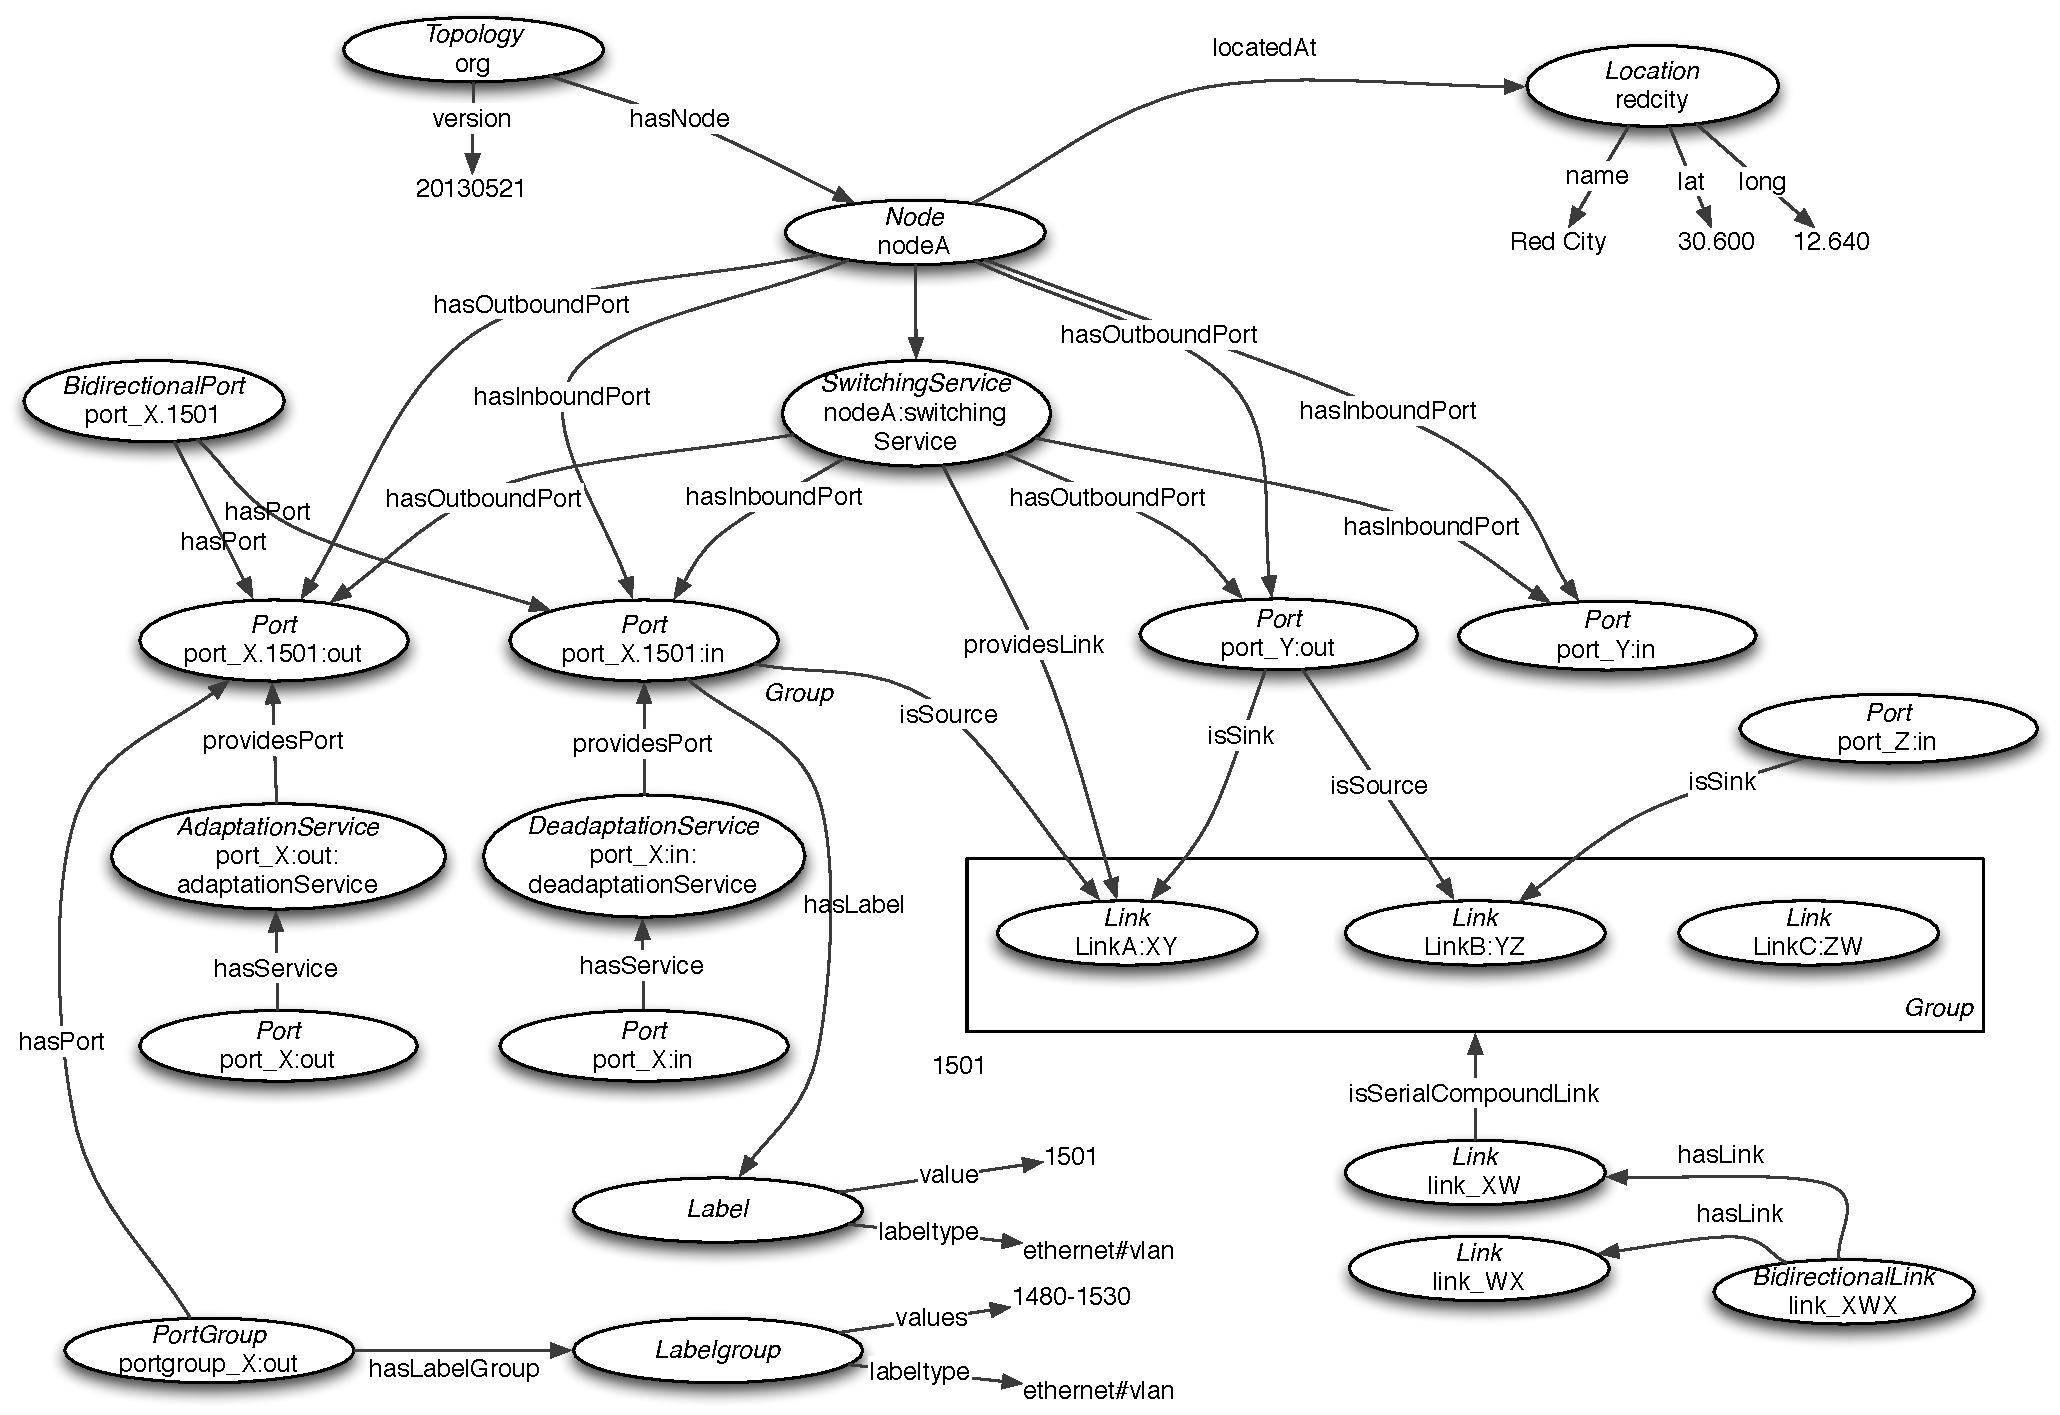
\includegraphics[width=\textwidth,angle=90]{combined-examples.pdf}
    \caption{A graphical overview showing the combination of all examples}
    \label{fig:combined-examples}
\end{figure}

\subsection{Examples in XML}
The following snippets represent NML structures in the XML format.

\begin{itemize}

    \item \emph{Topology} (section~\ref{class:topology})
      \lstinputlisting{xml/example-topology.xml}
    \item \emph{Node} (section~\ref{class:node})
      \lstinputlisting{xml/example-node.xml}
    \item \emph{Ports}  
      \begin{itemize}
        \item \emph{(Unidirectional) Port}  (section~\ref{class:port})
          \lstinputlisting{xml/example-port-unidir.xml}
        \item \emph{BidirectionalPort} (section~\ref{class:bidirectional_port})
          \lstinputlisting{xml/example-port-bidir.xml}
        \item \emph{PortGroup} (section~\ref{class:port_group})
          \lstinputlisting{xml/example-portgroup.xml}
      \end{itemize}
    \item \emph{Links} 
      \begin{itemize}
        \item \emph{UnidirectionalLink} (external) (section~\ref{class:link})
          \lstinputlisting{xml/example-link-unidir.xml}
        \item \emph{UnidirectionalLink} (internal) (section~\ref{class:link})
          \lstinputlisting{xml/example-link-unidir-cc.xml}
        \item \emph{UnidirectionalLink that is composed of more than one sub-link}
          \lstinputlisting{xml/example-link-serialcompound.xml}
        \item \emph{BidirectionalLink} (section~\ref{class:bidirectional_link})
          \lstinputlisting{xml/example-link-bidir.xml}
        \item \emph{LinkGroup} (section~\ref{class:link_group})
          \lstinputlisting{xml/example-linkgroup.xml}
      \end{itemize}
    \item \emph{Labels}
      \begin{itemize}
        \item \emph{Label} (section~\ref{class:label})
          \lstinputlisting{xml/example-label.xml}
        \item \emph{LabelGroup} (section~\ref{class:label_group})
          \lstinputlisting{xml/example-labelgroup.xml}
      \end{itemize}
    \item \emph{Location} (section~\ref{class:location})
      \lstinputlisting{xml/example-location.xml}
    \item \emph{Services}
      \begin{itemize}
        \item \emph{SwitchingService} (section~\ref{class:switching_service})
          \lstinputlisting{xml/example-switchingservice.xml}
        \item \emph{AdaptationService} (section~\ref{class:adaptation_service})
          \lstinputlisting{xml/example-adaptationservice.xml}
        \item \emph{DeadaptationService} (section~\ref{class:deadaptation_service})
          \lstinputlisting{xml/example-deadaptationservice.xml}
      \end{itemize}

\end{itemize}

\pagebreak

\subsection{Examples in OWL}
The following snippets represent NML structures in the OWL format.
The namespaces used in all the examples follow the definitions of the Topology example.

\begin{itemize}

    \item \emph{Topology} (section~\ref{class:topology})
      \lstinputlisting{owl/example-topology.xml}
    \item \emph{Node} (section~\ref{class:node})
      \lstinputlisting{owl/example-node.xml}
    \item \emph{Ports}  
      \begin{itemize}
        \item \emph{(Unidirectional) Port}  (section~\ref{class:port})
          \lstinputlisting{owl/example-port-unidir.xml}
        \item \emph{BidirectionalPort} (section~\ref{class:bidirectional_port})
          \lstinputlisting{owl/example-port-bidir.xml}
        \item \emph{PortGroup} (section~\ref{class:port_group})
          \lstinputlisting{owl/example-portgroup.xml}
      \end{itemize}
    \item \emph{Links} 
      \begin{itemize}
        \item \emph{UnidirectionalLink} (external) (section~\ref{class:link})
          \lstinputlisting{owl/example-link-unidir.xml}
        \item \emph{UnidirectionalLink} (internal) (section~\ref{class:link})
          \lstinputlisting{owl/example-link-unidir-cc.xml}
        \item \emph{UnidirectionalLink that is composed of more than one sub-link}
          \lstinputlisting{owl/example-link-serialcompound.xml}
        \item \emph{BidirectionalLink} (section~\ref{class:bidirectional_link})
          \lstinputlisting{owl/example-link-bidir.xml}
        \item \emph{LinkGroup} (section~\ref{class:link_group})
          \lstinputlisting{owl/example-linkgroup.xml}
      \end{itemize}
    \item \emph{Labels}
      \begin{itemize}
        \item \emph{Label} (section~\ref{class:label})
          \lstinputlisting{owl/example-label.xml}
        \item \emph{LabelGroup} (section~\ref{class:label_group})
          \lstinputlisting{owl/example-labelgroup.xml}
      \end{itemize}
    \item \emph{Location} (section~\ref{class:location})
      \lstinputlisting{owl/example-location.xml}
    \item \emph{Services}
      \begin{itemize}
        \item \emph{SwitchingService} (section~\ref{class:switching_service})
          \lstinputlisting{owl/example-switchingservice.xml}
        \item \emph{AdaptationService} (section~\ref{class:adaptation_service})
          \lstinputlisting{owl/example-adaptationservice.xml}
        \item \emph{DeadaptationService} (section~\ref{class:deadaptation_service})
          \lstinputlisting{owl/example-deadaptationservice.xml}
      \end{itemize}

\end{itemize}

\subsection{Conceptual Examples}

This section shows a few examples how NML was designed to be used. Like the other examples, this section is informative.  It may be possible that there are other ways to use the NML objects and attributes.

\subsubsection{Topology and Node}

A \emph{Topology} and \emph{Node} behave similar: they both contain inbound ports and outbound ports, and can contain a \emph{SwitchingService} to allow creation of internal links (cross connects) from inbound ports to outbound ports. Especially with the ability to create logical, sliced or virtual devices, the distinction is getting blurred.

The distinction is that a \emph{Node} is located at a single geographic location, while a \emph{Topology} is a set of geographically disperse Network Objects.

\subsubsection{Hierarchical Topology}

Large networks may want to publish both details of their network topology as a whole, as well as details about regional segments, without publishing details of the actual devices. NML allows the publication of a hierarchical \emph{Topology} tree, where the top-level \emph{Topology} has a \emph{hasTopology} relation with smaller \emph{Topologies}. These smaller Topologies must be fully enclosed -- the \emph{hasTopology} relation can not be used to relate partial overlapping Topologies.

For example, a \emph{Topology} \texttt{A} may want to publish about two parts of its Topology, \texttt{A\_West}, and \texttt{A\_East}. This allows it to publish difference in connectivity and costs between the two parts. It can do so with the following relations:

\nmlrelation{Topology \texttt{A}}{}{hasTopology}{}{Topology \texttt{A\_West}}\\
\nmlrelation{Topology \texttt{A}}{}{hasTopology}{}{Topology \texttt{A\_East}}

\subsubsection{Links, Segments and Paths}

A \emph{Link} object can refer to any link connection. A link segment and an end-to-end path are both described by a \emph{Link} object. This is by design, since it is easy to extend a \emph{Link}, or to describe a partition of a \emph{Link}.

Figure~\ref{fig:compound-link} gives an example of three different partitionings of a link between \texttt{port\_X:in} and \texttt{port\_W:out}.

\begin{figure}[htb]
    \centering
        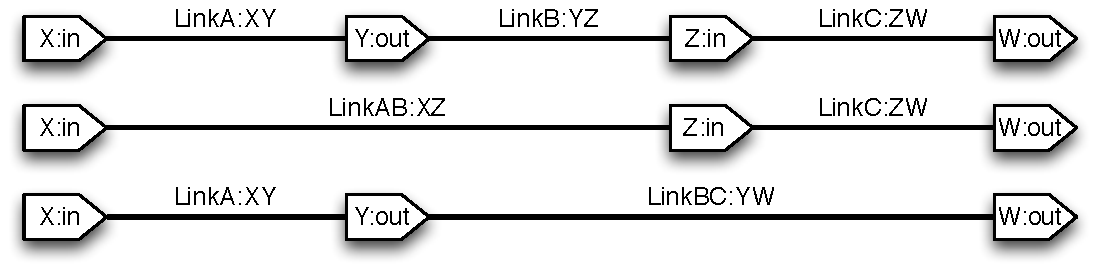
\includegraphics[width=.8\textwidth]{compound-link.pdf}
    \caption{Different partitionings of the same link.}
    \label{fig:compound-link}
\end{figure}

Note that in this example Port \texttt{port\_Y:out} is the source of both \texttt{linkB:YZ} and of \texttt{linkBC:YW}. If a single topology description would contain the full link and the partitioning, a path finding algoritm \MUST{} be aware that the fact that if a Port is the source of two NML Links, this does not mean it multicast to different network links. For this reason, it is \RECOMMENDED{} that applications either add metadata about the type of link, or specify that in certain messages, only one particular type of Link \MUST{} be used.


\subsubsection{Patch Panel and Media Convertor}

A port on a patch panel or optical distribution frame can simply be described as a NML Port (thus without an associated Node):

\nmlrelation{Port \texttt{odf\_X}}{}{isSink}{}{Link \texttt{A}}\\
\nmlrelation{Port \texttt{odf\_X}}{}{isSource}{}{Link \texttt{B}}

A mediaconvertor, e.g. from Ethernet over UTP to Ethernet over fiber, can be described in the same way, provided that the connected Links described the Ethernet connections. If the connected Links describe the underlying UTP and fiber connections, it is necessary to describe the conversion between them:

\nmlrelation{Port \texttt{Port\_X\_UTP}}{}{isSink}{}{Link \texttt{UTP\_A}} \\
\nmlrelation{Port \texttt{Port\_X\_fiber}}{}{isSource}{}{Link \texttt{fiber\_B}} \\
\nmlrelation{Port \texttt{Port\_X\_UTP}}{}{hasService}{}{DeAdaptataionService \texttt{X\_deadaptation}} \\
\nmlrelation{Port \texttt{Port\_X\_fiber}}{}{hasService}{}{AdaptationService \texttt{X\_adaptation}} \\
\nmlrelation{DeAdaptataionService \texttt{X\_deadaptation}}{}{providesPort}{}{Port \texttt{Port\_X\_eth}} \\
\nmlrelation{AdaptationService \texttt{X\_adaptation}}{}{providesPort}{}{Port \texttt{Port\_X\_eth}}


\subsubsection{VLAN and Broadcast Medium}

A VLAN is much like a broadcast medium, which can be described as a multipoint-to-multipoint Link:

\nmlrelation{Port \texttt{Port\_X:in}}{}{isSink}{}{Link \texttt{VLAN\_42}} \\
\nmlrelation{Port \texttt{Port\_X:out}}{}{isSink}{}{Link \texttt{VLAN\_42}} \\
\nmlrelation{Port \texttt{Port\_Y:in}}{}{isSink}{}{Link \texttt{VLAN\_42}} \\
\nmlrelation{Port \texttt{Port\_Y:out}}{}{isSink}{}{Link \texttt{VLAN\_42}} \\
\nmlrelation{Port \texttt{Port\_Z:in}}{}{isSink}{}{Link \texttt{VLAN\_42}} \\
\nmlrelation{Port \texttt{Port\_Z:out}}{}{isSink}{}{Link \texttt{VLAN\_42}} \\

Where \texttt{X}, \texttt{Y} and \texttt{Z} are in fact bidirectional ports:

\nmlrelation{BidirectionalPort \texttt{Port\_X}}{}{hasPort}{}{Port \texttt{Port\_X:in}} \\
\nmlrelation{BidirectionalPort \texttt{Port\_X}}{}{hasPort}{}{Port \texttt{Port\_X:out}} \\
\nmlrelation{BidirectionalPort \texttt{Port\_Y}}{}{hasPort}{}{Port \texttt{Port\_Y:in}} \\
\nmlrelation{BidirectionalPort \texttt{Port\_Y}}{}{hasPort}{}{Port \texttt{Port\_Y:out}} \\
\nmlrelation{BidirectionalPort \texttt{Port\_Z}}{}{hasPort}{}{Port \texttt{Port\_Z:in}} \\
\nmlrelation{BidirectionalPort \texttt{Port\_Z}}{}{hasPort}{}{Port \texttt{Port\_Z:out}} \\

However, this is not entirely correct: in the above description data coming from \texttt{Port\_X:in} would also be forwarded to \texttt{Port\_X:out}. However, the Ethernet technology prevents data returning on the same interface.

NML introduced the \emph{noReturnTraffic} parameter to describe this technological restriction: if the \emph{noReturnTraffic} parameter of a Link is true, there is no data transport from a source to a sink if the source and sink are grouped together in a BidirectionalPort group.

\nmlrelation{Link VLAN\_42}{}{noReturnTraffic}{}{"\texttt{true}"} \\


\subsubsection{Configuration and Potential Capability}

NML is able to both describe the network services (potential capability) as well as the network configuration.

A switching service can be described by a SwitchingService object along with associated inbound ports and outbound ports:

\nmlrelation{SwitchingService \texttt{switchmatrix\_A}}{}{hasInboundPort}{}{PortGroup \texttt{Port\_X:in}} \\
\nmlrelation{SwitchingService \texttt{switchmatrix\_A}}{}{hasOutboundPort}{}{PortGroup \texttt{Port\_X:out}} \\
\nmlrelation{SwitchingService \texttt{switchmatrix\_A}}{}{hasInboundPort}{}{PortGroup \texttt{Port\_Y:in}} \\
\nmlrelation{SwitchingService \texttt{switchmatrix\_A}}{}{hasOutboundPort}{}{PortGroup \texttt{Port\_Y:out}} \\
\nmlrelation{SwitchingService \texttt{switchmatrix\_A}}{}{labelSwapping}{}{\texttt{true}}

A cross connect created by this switching service can be specified by a Link object:

\nmlrelation{SwitchingService \texttt{switchmatrix\_A}}{}{providesLink}{}{Link \texttt{crossconnect\_A.1501}} \\
\nmlrelation{PortGroup \texttt{Port\_X:in}}{}{hasPort}{}{Port \texttt{Port\_X.1501:in}} \\
\nmlrelation{PortGroup \texttt{Port\_Y:out}}{}{hasPort}{}{Port \texttt{Port\_Y.1501:out}} \\
\nmlrelation{Port \texttt{Port\_X.1501:in}}{}{isSource}{}{Link \texttt{crossconnect\_A.1501}} \\
\nmlrelation{Port \texttt{Port\_Y.1501:out}}{}{isSink}{}{Link \texttt{crossconnect\_A.1501}}

An encoding and decoding service can be described by a AdapdationService and DeAdaptationService:

\nmlrelation{Port \texttt{Port\_X\_fiber:in}}{}{hasService}{}{DeAdaptationService \texttt{port\_X:in:deadaptation}} \\
\nmlrelation{DeAdaptationService \texttt{port\_X:in:deadaptation}}{}{canProvidePort}{}{PortGroup \texttt{Port\_X:in}}

A channel created by this encoding service can be specified by a \emph{providesPort} relation:

\nmlrelation{DeAdaptationService \texttt{port\_X:in:deadaptation}}{}{providesPort}{}{Port \texttt{Port\_X.1501:in}} \\
\nmlrelation{PortGroup \texttt{Port\_X:in}}{}{hasPort}{}{Port \texttt{Port\_X.1501:in}}


\subsubsection{Versioning and Lifetime}

The version of a \emph{Topology} indicated the serial number. If there are two \emph{Topology} descriptions for the same network, the one with the highest version number is the most recent version. The \emph{LifeTime} object is used to indicate when a certain resource is available.

Imagine that a link will have a scheduled downtime due to maintenance next week between 2 AM and 4 AM. This can be specified with these relations:

\nmlrelation{Topology \texttt{org}}{}{version}{}{\texttt{20130521T000000Z}} \\
\nmlrelation{Link \texttt{A}}{}{existsDuring}{}{LifeTime \texttt{A\_lifetime1}} \\
\nmlrelation{Link \texttt{A}}{}{existsDuring}{}{LifeTime \texttt{A\_lifetime2}} \\
\nmlrelation{LifeTime \texttt{A\_lifetime1}}{}{end}{}{\texttt{20130611T020000Z}} \\
\nmlrelation{LifeTime \texttt{A\_lifetime2}}{}{start}{}{\texttt{20130611T040000Z}}

Imagine that this planned maintainance is rescheduled. That can be specified by creating a new Topology with a new version number, and updated data:

\nmlrelation{Topology \texttt{org}}{}{version}{}{\texttt{20130604T000000Z}} \\
\nmlrelation{Link \texttt{A}}{}{existsDuring}{}{LifeTime \texttt{A\_lifetime1}} \\
\nmlrelation{Link \texttt{A}}{}{existsDuring}{}{LifeTime \texttt{A\_lifetime2}} \\
\nmlrelation{LifeTime \texttt{A\_lifetime1}}{}{end}{}{\texttt{20130618T020000Z}} \\
\nmlrelation{LifeTime \texttt{A\_lifetime2}}{}{start}{}{\texttt{20130618T040000Z}}


